\documentclass[aspectratio=169]{beamer}
\usepackage{UAH-theme}
\usepackage{minted}
\usepackage{xcolor}
% Use a placeholder if you don't have the actual logo
% Create a simple UAH logo placeholder
\usepackage{tikz}
\usepackage{array}
\usepackage{multirow}
\usepackage{array}
\usepackage{colortbl}
\usepackage{booktabs}
\usepackage{graphicx} 
\usepackage[many]{tcolorbox}


\usetikzlibrary{arrows.meta, positioning}
\definecolor{stackaddr}{RGB}{173,216,230}
\definecolor{stackval}{RGB}{255,228,181}
\definecolor{stackdesc}{RGB}{144,238,144}
\definecolor{addr}{RGB}{173,216,230}
\definecolor{val}{RGB}{255,228,181}
\definecolor{desc}{RGB}{144,238,144}

\newcommand{\UAHLogoPlaceholder}{%
\begin{tikzpicture}[scale=0.15]
\draw[fill=UAHred,draw=none] (0,0) circle (5);
\draw[white,line width=0.5mm] (0,0) circle (4);
\draw[white,line width=0.5mm] (-2,2) -- (2,2);
\draw[white,line width=0.5mm] (-2,-2) -- (2,-2);
\draw[white,line width=0.5mm] (0,4) -- (0,-4);
\end{tikzpicture}%
}

\definecolor{frame1}{RGB}{255, 230, 230}
\definecolor{frame2}{RGB}{230, 255, 230}
\definecolor{frame3}{RGB}{230, 230, 255}
\definecolor{frame4}{RGB}{255, 255, 230}

\definecolor{androidBlue}{HTML}{8AB4F8}
\definecolor{androidBlueLight}{HTML}{E8F0FE}
\definecolor{androidGreen}{HTML}{81C995}
\definecolor{androidGreenLight}{HTML}{E6F4EA}

% Red variants - based on Android's "error" and warning colors
\definecolor{androidRed}{HTML}{F28B82}
\definecolor{androidRedLight}{HTML}{FADAD7}

% Yellow variants - based on Android's accent/warning colors
\definecolor{androidYellow}{HTML}{FDD663}
\definecolor{androidYellowLight}{HTML}{FEF7E0}

% Purple variants - based on Android's system UI accents
\definecolor{androidPurple}{HTML}{D7AEFB}
\definecolor{androidPurpleLight}{HTML}{F4EAFC}

% Orange variants - based on Android's notification colors
\definecolor{androidOrange}{HTML}{FCAD70}
\definecolor{androidOrangeLight}{HTML}{FEEADC}

% Teal variants - based on Android's Material You palette
\definecolor{androidTeal}{HTML}{78D9EC}
\definecolor{androidTealLight}{HTML}{E6F6F9}

% Gray variants - based on Android's neutral colors
\definecolor{androidGray}{HTML}{DADCE0}
\definecolor{androidGrayLight}{HTML}{F1F3F4}



\usemintedstyle{default}
\setminted{
fontsize=\footnotesize,
frame=single,
linenos=true,
breaklines=true,
autogobble=true
}


\title{08A ARM Machine Code: Data Processing Instructions}
\subtitle{CPE 221}
\author{Rahul Bhadani}
\institute{The University of Alabama in Huntsville}
\date{\today}


\begin{document}

\begin{frame}

    \titlepage

\end{frame}

\begin{frame}{Table of Content}
    \tableofcontents
\end{frame}


\begin{frame}{Data Processing Instructions}
\begin{center}
    % Instruction format table
    \begin{tabular}{|p{4em}|p{4em}|p{4em}|p{4em}|p{4em}|p{4em}|}
    \hline
    31:28 & 27:26 & 25:20 & 19:16 & 15:12 & 11:0 \\
    \hline
    cond & op & funct & Rn & Rd & Src2 \\
    \hline
    4 bits & 2 bits & 6 bits & 4 bits & 4 bits & 12 bits \\
    \hline
    \end{tabular}

    \vspace{0.5cm}

    \begin{tabular}{|p{11em}|p{11em}|p{11em}|}
        \hline
        Bit 25 & Bits 24:21 & Bit 20\\
        \hline
        I & cmd & S \\
        \hline
        I = 1 when Src2 is an immediate & Specific data-processing instruction & S= 1 when an instruction sets the condition flags\\
        \hline
    \end{tabular}
\end{center}

\end{frame}

\section{Encoding Immediates in ARM Assembly}

\begin{frame}
    \sectionpage
\end{frame}


\begin{frame}{Encoding Immediates for Data Processing Instructions}
    \begin{center}
        % Instruction format table
        \begin{tabular}{|p{4em}|p{4em}|p{4em}|p{4em}|p{4em}|p{4em}|}
        \hline
        31:28 & 27:26 & 25:20 & 19:16 & 15:12 & 11:0 \\
        \hline
        cond & op & funct & Rn & Rd & Src2 \\
        \hline
        \end{tabular}

        \vspace{0.5cm}


        \begin{tabular}{|p{11em}|p{11em}|}
            \hline
            Bit 11:8 & Bits 7:0\\
            \hline
            rot & imm8 \\
            \hline
        \end{tabular}

        \vspace{0.5cm}

        imm8 = 8-bit immediate

        rot = 4-bit rotation

        imm8 is rotated right by 2 $\times$ rot to create a 32-bit constant.


    \end{center}

\end{frame}

% https://alisdair.mcdiarmid.org/arm-immediate-value-encoding/

\begin{frame}{4-bit Rotation, 8-bit Immediate}

    ARM doesn't use the 12-bit immediate value as a 12-bit number. Instead, it's an 8-bit number with a 4-bit rotation, like this:


    \vspace{0.5cm}

    \begin{tabular}{|p{11em}|p{11em}|}
        \hline
        Bit 11:8 & Bits 7:0\\
        \hline
        rot & imm8 \\
        \hline
    \end{tabular}


    \vspace{0.5cm}

    The 4-bit rotation value has 16 possible settings (i.e. 0, 2, 4, 6, 8, 10, 12, 14, 16, 18, 20, 22, 24, 26, 28, 30), so it's not possible to rotate the 8-bit value to any position in the 32-bit word. The most useful way to use this rotation value is to multiply it by two. It can then represent all even numbers from zero to 30.
    
\end{frame}

\begin{frame}{4-bit Rotation, 8-bit Immediate}
    To form the constant for the data processing instruction, the 8-bit immediate value is extended with zeroes to 32 bits, then rotated the specified number of places to the right. For some values of rotation, this can allow splitting the 8-bit value between bytes. See the table in the next slide for all possible rotations.

\end{frame}

\begin{frame}{}

    \begin{center}
        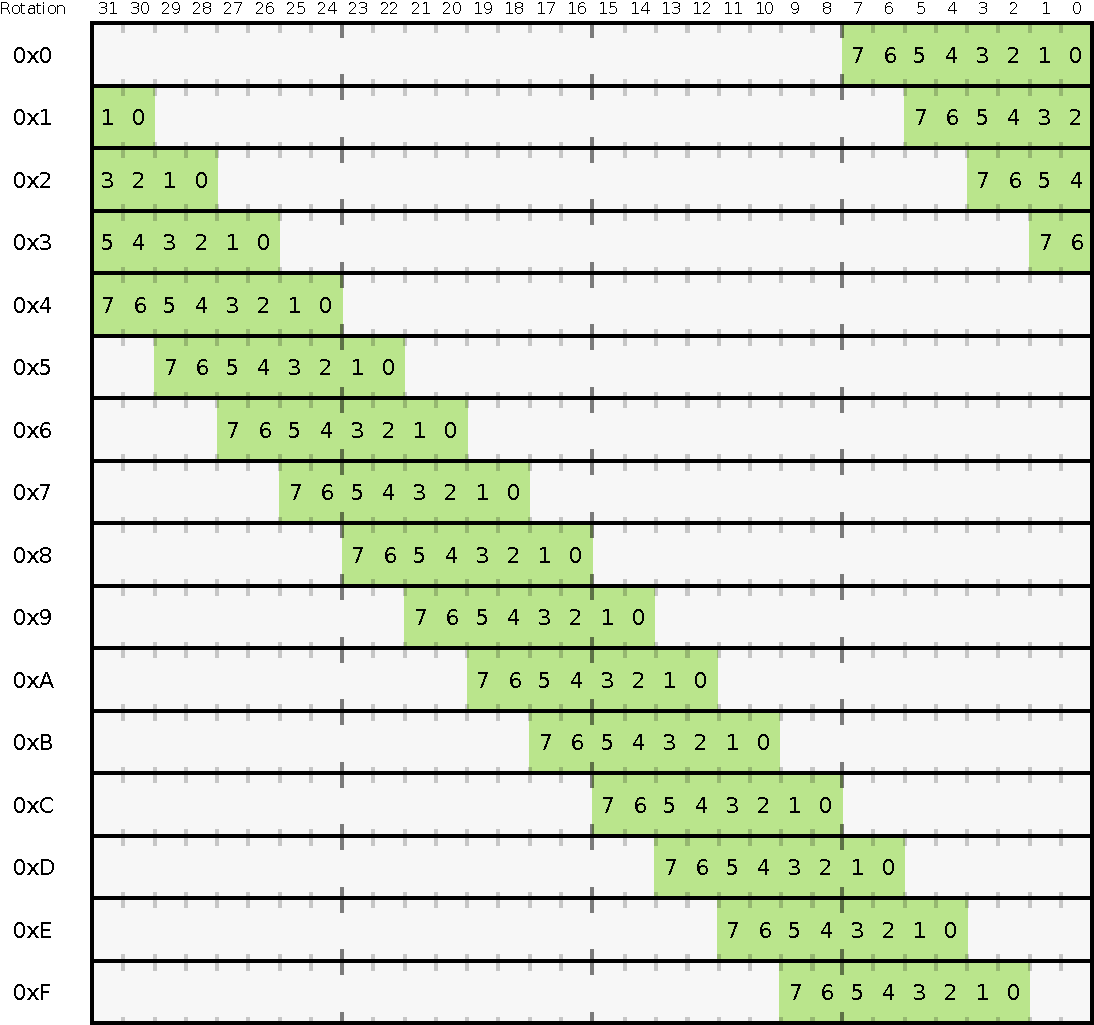
\includegraphics[width=0.62\linewidth]{../figures/possiblerotations.pdf}
    \end{center}
    
\end{frame}
\begin{frame}{Example 1}
    
    \begin{tcolorbox}[
        enhanced,
        colback=androidBlueLight,
        colframe=androidBlue,
        arc=5pt,
        boxrule=1pt,
        title=\textbf{},
        fonttitle=\bfseries,
        coltitle=black,
        top=10pt,
        bottom=8pt,
        left=8pt,
        right=8pt,
        attach boxed title to top left={xshift=10pt, yshift=-\tcboxedtitleheight/2},
        boxed title style={
        colback=androidBlue,    
            colframe=androidBlue,
            arc=3pt,
            boxrule=0pt,
            left=6pt, right=6pt,
            top=3pt, bottom=3pt
        }
        ]
        Encode   \texttt{SUB R2, R3, 0xFF0}
    \end{tcolorbox}

    \begin{itemize}
        \item \texttt{0xFF0 = 1111 1111 0000}
        \item It is 12 bits but need to find a way to represent using 8 bits.
        \item Given, 0XFF0, we first write it as 32-bit: 0x00000FF0 which is
        
        0000 0000 0000 0000 0000 1111 1111 0000
        \item Since the above number cannot be accomodated in 8 bits (minimum need is 12 bits), we need to rotate it.
        \item By looking at the table in the previous slide, we see that 0000 0000 0000 0000 0000 1111 1111 0000 is corresponding to 0xE which means we need 14 $\times$ 2 = 28 rotation.
        \item Hence rot = 1110, imm8 = 1111 1111
    \end{itemize}
    
\end{frame}

\begin{frame}{Note}
    Not all 32 bits can be represented by the above logic, so not all immediates greater than 8 bits are valid immediates.
\end{frame}

\section{Encoding Shift Instructions}

\begin{frame}
    \sectionpage
\end{frame}

\begin{frame}{Encoding Shift Instructions}
    
    \begin{center}
        % Instruction format table
        \begin{tabular}{|p{4em}|p{4em}|p{4em}|p{4em}|p{4em}|p{4em}|}
        \hline
        31:28 & 27:26 & 25:20 & 19:16 & 15:12 & 11:0 \\
        \hline
        cond & op & funct & Rn & Rd & Src2 \\
        \hline
        4 bits & 2 bits & 6 bits & 4 bits & 4 bits & 12 bits \\
        \hline
        \end{tabular}
    
        \vspace{0.5cm}
    
        \begin{tabular}{|p{13em}|p{9em}|p{11em}|}
            \hline
            Bit 25 & Bits 24:21 & Bit 20\\
            \hline
            I & cmd & S \\
            \hline
            I = 0 for LSL, LSR, ROR, ASR 
            
            I = 1 for MOV
            & 1101 & S= 1 when an instruction sets the condition flags\\
            \hline
        \end{tabular}
    \end{center}

\end{frame}

\begin{frame}{Encoding Shift Instructions: Register Value Shift by Constant}
    
    Register Value Shift by Constant or Immediate (Shift Amount)
    
    \begin{center}
        % Instruction format table
        \begin{tabular}{|p{4em}|p{4em}|p{4em}|p{4em}|p{4em}|p{4em}|}
        \hline
        31:28 & 27:26 & 25:20 & 19:16 & 15:12 & 11:0 \\
        \hline
        cond & op & funct & Rn & Rd & Src2 \\
        \hline
        4 bits & 2 bits & 6 bits & 4 bits & 4 bits & 12 bits \\
        \hline
        \end{tabular}
    
        \vspace{0.5cm}
    
        LSL/LSR/ASR/ROR Rd,  Rm, shamt5

        \vspace{0.5cm}
    
\begin{columns}
    \column{0.7\linewidth}
    \begin{tabular}{|p{4em}|p{4em}|p{4em}|p{4em}|}
        \hline
        Bits 11:7 & Bits 6:5 & Bit 4 &  Bits 3:0 \\
        \hline
        shamt5 & sh & 0 &  Rm  \\
        \hline
    \end{tabular} 

    \vspace{0.5cm}

    shamt5 = a constant by which the register Rm is shifted

    \column{0.3\linewidth}

    \begin{tabular}{|p{2em}|p{6em}|}
        \hline
        sh & Instructions\\
        \hline
        00 & LSL\\ \hline
        01 & LSR \\ \hline
        10 & ASR \\ \hline
        11 & ROR \\ \hline
    \end{tabular}

\end{columns}
        
\end{center}
\end{frame}

\begin{frame}{Example 2}
    
    \begin{tcolorbox}[
        enhanced,
        colback=androidBlueLight,
        colframe=androidBlue,
        arc=5pt,
        boxrule=1pt,
        title=\textbf{},
        fonttitle=\bfseries,
        coltitle=black,
        top=10pt,
        bottom=8pt,
        left=8pt,
        right=8pt,
        attach boxed title to top left={xshift=10pt, yshift=-\tcboxedtitleheight/2},
        boxed title style={
        colback=androidBlue,    
            colframe=androidBlue,
            arc=3pt,
            boxrule=0pt,
            left=6pt, right=6pt,
            top=3pt, bottom=3pt
        }
        ]
        Encode     \texttt{LSL R3, R2, \#23}
    \end{tcolorbox}

    \begin{center}
        % Instruction format table
        \begin{tabular}{|p{4em}|p{4em}|p{4em}|p{4em}|p{4em}|p{4em}|}
        \hline
        31:28 & 27:26 & 25:20 & 19:16 & 15:12 & 11:0 \\
        \hline
        1110 & 00 & 0 1101 0 & 0000 & 0011 & Src2 \\
        \hline
        4 bits & 2 bits & 6 bits & 4 bits & 4 bits & 12 bits \\
        \hline
        \end{tabular}
    
        \vspace{0.5cm}
    
        \vspace{0.5cm}
    
\begin{columns}
    \column{0.7\linewidth}
    \textbf{Src2:}

    \vspace{0.3cm}

    \begin{tabular}{|p{4em}|p{4em}|p{4em}|p{4em}|}
        \hline
        Bits 11:7 & Bits 6:5 & Bit 4 &  Bits 3:0 \\
        \hline
        10111 & 00 & 0 &  0010  \\
        \hline
    \end{tabular} 

    \vspace{0.5cm}

    \column{0.3\linewidth}

\end{columns}
        
\end{center}
    
    
\end{frame}

\begin{frame}{Example 3}
    
    \begin{tcolorbox}[
        enhanced,
        colback=androidBlueLight,
        colframe=androidBlue,
        arc=5pt,
        boxrule=1pt,
        title=\textbf{},
        fonttitle=\bfseries,
        coltitle=black,
        top=10pt,
        bottom=8pt,
        left=8pt,
        right=8pt,
        attach boxed title to top left={xshift=10pt, yshift=-\tcboxedtitleheight/2},
        boxed title style={
        colback=androidBlue,    
            colframe=androidBlue,
            arc=3pt,
            boxrule=0pt,
            left=6pt, right=6pt,
            top=3pt, bottom=3pt
        }
        ]
        Encode      \texttt{MOV R3, R2}
    \end{tcolorbox}

    \begin{center}
        % Instruction format table
        \begin{tabular}{|p{4em}|p{4em}|p{4em}|p{4em}|p{4em}|p{4em}|}
        \hline
        31:28 & 27:26 & 25:20 & 19:16 & 15:12 & 11:0 \\
        \hline
        1110 & 00 & 1 1101 0 & 0000 & 0011 & Src2 \\
        \hline
        4 bits & 2 bits & 6 bits & 4 bits & 4 bits & 12 bits \\
        \hline
        \end{tabular}

        \vspace{0.5cm}
    
\begin{columns}
    \column{0.7\linewidth}
    \textbf{Src2:}

    \vspace{0.3cm}

    \begin{tabular}{|p{4em}|p{4em}|p{4em}|p{4em}|}
        \hline
        Bits 11:7 & Bits 6:5 & Bit 4 &  Bits 3:0 \\
        \hline
        00000 & 00 & 0 &  0010  \\
        \hline
    \end{tabular} 

    \vspace{0.5cm}

    \column{0.3\linewidth}

\end{columns}
        
\vspace{0.5cm}

1110 0011 1010 0000 0011 0000 0000 0010

0x E 3 A 0 3 0 0 2

\end{center}
    

\end{frame}

\begin{frame}{Example 4}
    
    \begin{tcolorbox}[
        enhanced,
        colback=androidBlueLight,
        colframe=androidBlue,
        arc=5pt,
        boxrule=1pt,
        title=\textbf{},
        fonttitle=\bfseries,
        coltitle=black,
        top=10pt,
        bottom=8pt,
        left=8pt,
        right=8pt,
        attach boxed title to top left={xshift=10pt, yshift=-\tcboxedtitleheight/2},
        boxed title style={
        colback=androidBlue,    
            colframe=androidBlue,
            arc=3pt,
            boxrule=0pt,
            left=6pt, right=6pt,
            top=3pt, bottom=3pt
        }
        ]
        Encode     \texttt{MOV R3, \#0xFF0}
    \end{tcolorbox}

    \begin{center}
        % Instruction format table
        \begin{tabular}{|p{4em}|p{4em}|p{4em}|p{4em}|p{4em}|p{4em}|}
        \hline
        31:28 & 27:26 & 25:20 & 19:16 & 15:12 & 11:0 \\
        \hline
        1110 & 00 & 1 1101 0 & 0000 & 0011 & Src2 \\
        \hline
        4 bits & 2 bits & 6 bits & 4 bits & 4 bits & 12 bits \\
        \hline
        \end{tabular}

        \vspace{0.5cm}
    
\begin{columns}
    \column{0.7\linewidth}
    \textbf{Src2:} follows the same convention as in Example 1.

    \vspace{0.5cm}

    \column{0.3\linewidth}

\end{columns}
        
\vspace{0.5cm}

1110 0011 1010 0000 0011 1110 1111 1111

0x E 3 A 0 3 E F F

\end{center}
    

\end{frame}


\begin{frame}{Encoding Shift Instructions: Register Value Shift by Register Value}
    
    Register Value Shift by Constant or Immediate (Shift Amount)
    
    \begin{center}
        % Instruction format table
        \begin{tabular}{|p{4em}|p{4em}|p{4em}|p{4em}|p{4em}|p{4em}|}
        \hline
        31:28 & 27:26 & 25:20 & 19:16 & 15:12 & 11:0 \\
        \hline
        cond & op & funct & Rn & Rd & Src2 \\
        \hline
        4 bits & 2 bits & 6 bits & 4 bits & 4 bits & 12 bits \\
        \hline
        \end{tabular}
    
        \vspace{0.5cm}
    
        LSL/LSR/ASR/ROR Rd,  Rm, Rs

        \vspace{0.5cm}
    
\begin{columns}
    \column{0.7\linewidth}
    \begin{tabular}{|p{4em}|p{4em}|p{4em}|p{4em}|p{4em}|}
        \hline
        Bits 11:8 & Bit 7 & Bits 6:5 &  Bit 4 & Bits 3:0 \\
        \hline
        Rs & 0 & sh &  1 & Rm  \\
        \hline
    \end{tabular} 

    \vspace{0.5cm}

    \column{0.3\linewidth}

    \begin{tabular}{|p{2em}|p{6em}|}
        \hline
        sh & Instructions\\
        \hline
        00 & LSL\\ \hline
        01 & LSR \\ \hline
        10 & ASR \\ \hline
        11 & ROR \\ \hline
    \end{tabular}

\end{columns}
        
\end{center}
\end{frame}


\begin{frame}{Example 5}
    
    \begin{tcolorbox}[
        enhanced,
        colback=androidBlueLight,
        colframe=androidBlue,
        arc=5pt,
        boxrule=1pt,
        title=\textbf{},
        fonttitle=\bfseries,
        coltitle=black,
        top=10pt,
        bottom=8pt,
        left=8pt,
        right=8pt,
        attach boxed title to top left={xshift=10pt, yshift=-\tcboxedtitleheight/2},
        boxed title style={
        colback=androidBlue,    
            colframe=androidBlue,
            arc=3pt,
            boxrule=0pt,
            left=6pt, right=6pt,
            top=3pt, bottom=3pt
        }
        ]
        Encode 
        \texttt{ASR R3, R5, R7}
    \end{tcolorbox}

    \begin{center}
        % Instruction format table
        \begin{tabular}{|p{4em}|p{4em}|p{4em}|p{4em}|p{4em}|p{4em}|}
        \hline
        31:28 & 27:26 & 25:20 & 19:16 & 15:12 & 11:0 \\
        \hline
        1110 & 00 & 0 1101 0 & 0000 & 0011 & Src2 \\
        \hline
        4 bits & 2 bits & 6 bits & 4 bits & 4 bits & 12 bits \\
        \hline
        \end{tabular}
    
        \vspace{0.5cm}
    
        \vspace{0.5cm}
    
\begin{columns}
    \column{0.7\linewidth}
    \textbf{Src2:}

    \vspace{0.3cm}

    \begin{tabular}{|p{4em}|p{4em}|p{4em}|p{4em}|p{4em}|}
        \hline
        Bits 11:8 & Bit 7 & Bits 6:5 & Bit 4 & Bits 3:0 \\
        \hline
        0111 & 0 & 10 &  1 & 0101  \\
        \hline
    \end{tabular} 

    \vspace{0.5cm}

    \column{0.3\linewidth}

\end{columns}
        
    1110 0001 1010 0000 0011 0111 0101 0101

    0x E 1 A 0 3 7 5 5

\end{center}
    

\end{frame}

\begin{frame}{Example 6}
    
    \begin{tcolorbox}[
        enhanced,
        colback=androidBlueLight,
        colframe=androidBlue,
        arc=5pt,
        boxrule=1pt,
        title=\textbf{},
        fonttitle=\bfseries,
        coltitle=black,
        top=10pt,
        bottom=8pt,
        left=8pt,
        right=8pt,
        attach boxed title to top left={xshift=10pt, yshift=-\tcboxedtitleheight/2},
        boxed title style={
        colback=androidBlue,    
            colframe=androidBlue,
            arc=3pt,
            boxrule=0pt,
            left=6pt, right=6pt,
            top=3pt, bottom=3pt
        }
        ]
        Encode 
        \texttt{ADD R7, R2, R3, LSL \#2}
    \end{tcolorbox}
Rn = R2, Rd = R7, Rm = R3
    \begin{center}
        % Instruction format table
        \begin{tabular}{|p{4em}|p{4em}|p{4em}|p{4em}|p{4em}|p{4em}|}
        \hline
        31:28 & 27:26 & 25:20 & 19:16 & 15:12 & 11:0 \\
        \hline
        1110 & 00 & 0 0100 0 & 0010 & 0111 & Src2 \\
        \hline
        4 bits & 2 bits & 6 bits & 4 bits & 4 bits & 12 bits \\
        \hline
        \end{tabular}
    
        \vspace{0.5cm}
    
        \begin{columns}
            \column{0.7\linewidth}
            \textbf{Src2:}
        
            \vspace{0.3cm}
        
            \begin{tabular}{|p{4em}|p{4em}|p{4em}|p{4em}|}
                \hline
                Bits 11:7 & Bits 6:5 & Bit 4 &  Bits 3:0 \\
                \hline
                00010 & 00 & 0 &  0011  \\
                \hline
            \end{tabular} 
        
            \vspace{0.3cm}
        
            \column{0.3\linewidth}
        
        \end{columns}
        
        1110    0000    1000    0010    0111    0001    0000    0011

    0x  E       0       8       2       7       1       0       3

\end{center}
    

\end{frame}


\section{Multiply Instructions}

\begin{frame}
    \sectionpage
\end{frame}

\begin{frame}{Multiply Instructions}
    \normalsize
    Multiply instructions use the encoding in below.
    The 3-bit \textit{cmd} field specifies the type of multiply, as given in in the Table.
    \vspace{0.5cm}
    \begin{center}
    {\large \textcolor{androidBlue}{Multiply}}
    \end{center}
    
    \begin{center}
    \footnotesize
    \begin{tabular}{|c|c|c|c|c|c|c|c|c|c|}
    \hline
    \multicolumn{1}{|c|}{31:28} & \multicolumn{1}{c|}{27:26} & \multicolumn{1}{c|}{25:24} & 
    \multicolumn{1}{c|}{23:21} & \multicolumn{1}{c|}{20} & \multicolumn{1}{c|}{19:16} & 
    \multicolumn{1}{c|}{15:12} & \multicolumn{1}{c|}{11:8} & \multicolumn{1}{|c|}{7:4} & \multicolumn{1}{c|}{3:0} \\
    \hline
    \textcolor{androidBlue}{cond} & \textcolor{androidBlue}{$\begin{array}{c}\text{op}\\00\end{array}$} & \textcolor{androidBlue}{00} & \textcolor{androidBlue}{cmd} & \textcolor{androidBlue}{S} & \textcolor{androidBlue}{Rd} & \textcolor{androidBlue}{Ra} & \textcolor{androidBlue}{Rm} & \textcolor{androidBlue}{1001} & \textcolor{androidBlue}{Rn}\\
    \hline
    4 bits & 2 bits & \multicolumn{2}{c}{6 bits} & \multicolumn{1}{c|}{} & 4 bits & 4 bits & 4 bits & 4 bits & 4 bits \\
    \cline{1-3}\cline{4-5}\cline{6-10}
    \end{tabular}
    
    \vspace{0.5cm}
    
    \vspace{0.3cm}
    \begin{flushright}
    \textbf{\textcolor{androidBlue}{} Multiply instruction encoding}
    \end{flushright}
    \end{center}
    \end{frame}
    
    \begin{frame}{Types of Multiply Instructions}
    \begin{center}
    \footnotesize
    \renewcommand{\arraystretch}{1.25} % Adjust this value as needed

    \begin{tabular}{|c|c|c|c|}
    \hline
    \rowcolor{androidBlue}\color{white}cmd & \color{white}Name & \color{white}Description & \color{white}Operation \\
    \hline
    000 & MUL Rd, Rn, Rm & Multiply & Rd $\leftarrow$ Rn $\times$ Rm (low 32 bits) \\
    \hline
    \rowcolor{androidBlueLight}001 & MLA Rd, Rn, Rm, Ra & \begin{tabular}{@{}c@{}}Multiply \\ Accumulate\end{tabular} & Rd $\leftarrow$ (Rn $\times$ Rm)+Ra (low 32 bits) \\
    \hline
    100 & UMULL Rd, Rn, Rm, Ra & \begin{tabular}{@{}c@{}}Unsigned Multiply \\ Long\end{tabular} & 
    \begin{tabular}{@{}l@{}}
    \{Rd, Ra\} $\leftarrow$ Rn $\times$ Rm \\
    (all 64 bits, Rm/Rn unsigned)
    \end{tabular} \\
    \hline
    \rowcolor{androidBlueLight}101 & UMLAL Rd, Rn, Rm, Ra & \begin{tabular}{@{}c@{}}Unsigned Multiply \\ Accumulate Long\end{tabular} & 
    \begin{tabular}{@{}l@{}}
    \{Rd, Ra\} $\leftarrow$ (Rn $\times$ Rm)+\{Rd, Ra\} \\
    (all 64 bits, Rm/Rn unsigned)
    \end{tabular} \\
    \hline
    110 & SMULL Rd, Rn, Rm, Ra & \begin{tabular}{@{}c@{}}Signed Multiply \\ Long\end{tabular} & 
    \begin{tabular}{@{}l@{}}
    \{Rd, Ra\} $\leftarrow$ Rn $\times$ Rm \\
    (all 64 bits, Rm/Rn signed)
    \end{tabular} \\
    \hline
    \rowcolor{androidBlueLight}111 & SMLAL Rd, Rn, Rm, Ra & \begin{tabular}{@{}c@{}}Signed Multiply \\ Accumulate Long\end{tabular} & 
    \begin{tabular}{@{}l@{}}
    \{Rd, Ra\} $\leftarrow$ (Rn $\times$ Rm)+\{Rd, Ra\} \\
    (all 64 bits, Rm/Rn signed)
    \end{tabular} \\
    \hline
    \end{tabular}
    \end{center}
    \end{frame}


    \begin{frame}
        \Huge{\centerline{\color{androidGreen}\textbf{The End}}}
    \end{frame}
    
\end{document}